The best way to quickly visualize the F-P model is to think in terms of a
persistent functional data structure with structural sharing. Then, rather than
containing pure data, imagine instead that the structure represents a directed
acyclic graph (DAG) of transformations on distributed data.

Importantly, since this DAG of computations is a persistent data structure
itself, it is safe to exchange (copies of) subgraphs of a DAG between remote
nodes. This enables a robust and easy-to-reason-about model of fault tolerance.
We call subgraphs of a DAG lineages; lineages enable restoring the data of
failed nodes through re-applying the transformations represented by their DAG.
This sequence of applications must begin with data available from stable
storage.

Central to our model is the careful use of laziness. Computations on
distributed data are typically not executed eagerly; instead, applying a
function to distributed data just creates an immutable lineage. To obtain the
result of a computation, it is necessary to first ``kick off'' computation, or
to force its lineage. Within our programming model, this force
operation\todo{which force operation?} makes network communication (and thus
possibilities for latency) explicit, which is considered to be a strength when
designing distributed systems~\cite{ANoteDistComp}. Deferred evaluation also
enables optimizing distributed computations through operation fusion, which
avoids the creation of unnecessary intermediate data structures--this is
efficient in time as well as space. This kind of optimization is particularly
important and effective in distributed systems~\cite{FlumeJava}.\todo{What does
this have to do with FlumeJava?}

\vspace{-3mm}
\begin{center}\noindent\rule{8cm}{0.4pt}\end{center}
\begin{displayquote}
For these reasons, we believe that laziness should be viewed as an enabler in
the design of distributed systems.
\end{displayquote}
\vspace{-4mm}
\begin{center}\noindent\rule{8cm}{0.4pt}\end{center}
\vspace{1mm}

\noindent The F-P model consists of three main components:
\begin{itemize}[noitemsep]
  \item {\bf Silos:} stationary typed data containers.
  \item {\bf SiloRefs:} references to local or remote Silos.
  \item {\bf Spores:} safe, serializable functions.
\end{itemize}
\vspace{1mm}

\paragraph{Silos}

A silo is a typed data container. It is stationary in the sense that it does
not move between machines -- it remains on the machine where it was created.
Data stored in a silo is typically loaded from stable storage, such as a
distributed file system. A program operating on data stored in a silo can only
do so using a reference to the silo, a \verb|SiloRef|.

\paragraph{SiloRefs}

Similar to a proxy object, a SiloRef represents, and allows interacting with,
both local and remote silos. SiloRefs are immutable, storing identifiers to
locate possibly remote silos. SiloRefs are also typed (\verb|SiloRef[T]|)
corresponding to the type of their silo's data, leading to well-typed network
communication. The SiloRef provides three primitive operations/combinators
(some are lazy, some are not): map, flatMap, and send. map lazily applies a
user-defined function to data pointed to by the SiloRef, creating in a new silo
containing the result of this application. Like map, flatMap lazily applies a
user-defined function to data pointed to by the SiloRef. Unlike map, the
user-defined function passed to flatMap returns a SiloRef whose contents is
transferred to the new silo returned by flatMap. Essentially, flatMap enables
accessing the contents of (local or remote) silos from within remote
computations. We illustrate these primitives in more detail in
Section~\ref{sec:primitives}.

\paragraph{Spores}

Spores~\cite{Spores} are safe closures that are guaranteed to be serializable
and thus distributable. They are a closure-like abstraction and type system
which gives authors of distributed frameworks a principled way of controlling
the environment which a closure (provided by client code) can capture. This is
achieved by (a) enforcing a specific syntactic shape which dictates how the
environment of a spore is declared, and (b) providing additional type-checking
to ensure that types being captured have certain properties.

\vspace{3mm}
\noindent A spore consists of two parts:

\begin{itemize}[noitemsep]
\item {\bf the spore header}, composed of a list of value definitions.
\item {\bf the spore body} (sometimes referred to as the “spore closure”), a
  regular closure.
\end{itemize}

\noindent This shape is illustrated below.

\vspace{-1mm}
\begin{figure}[h!]
\centering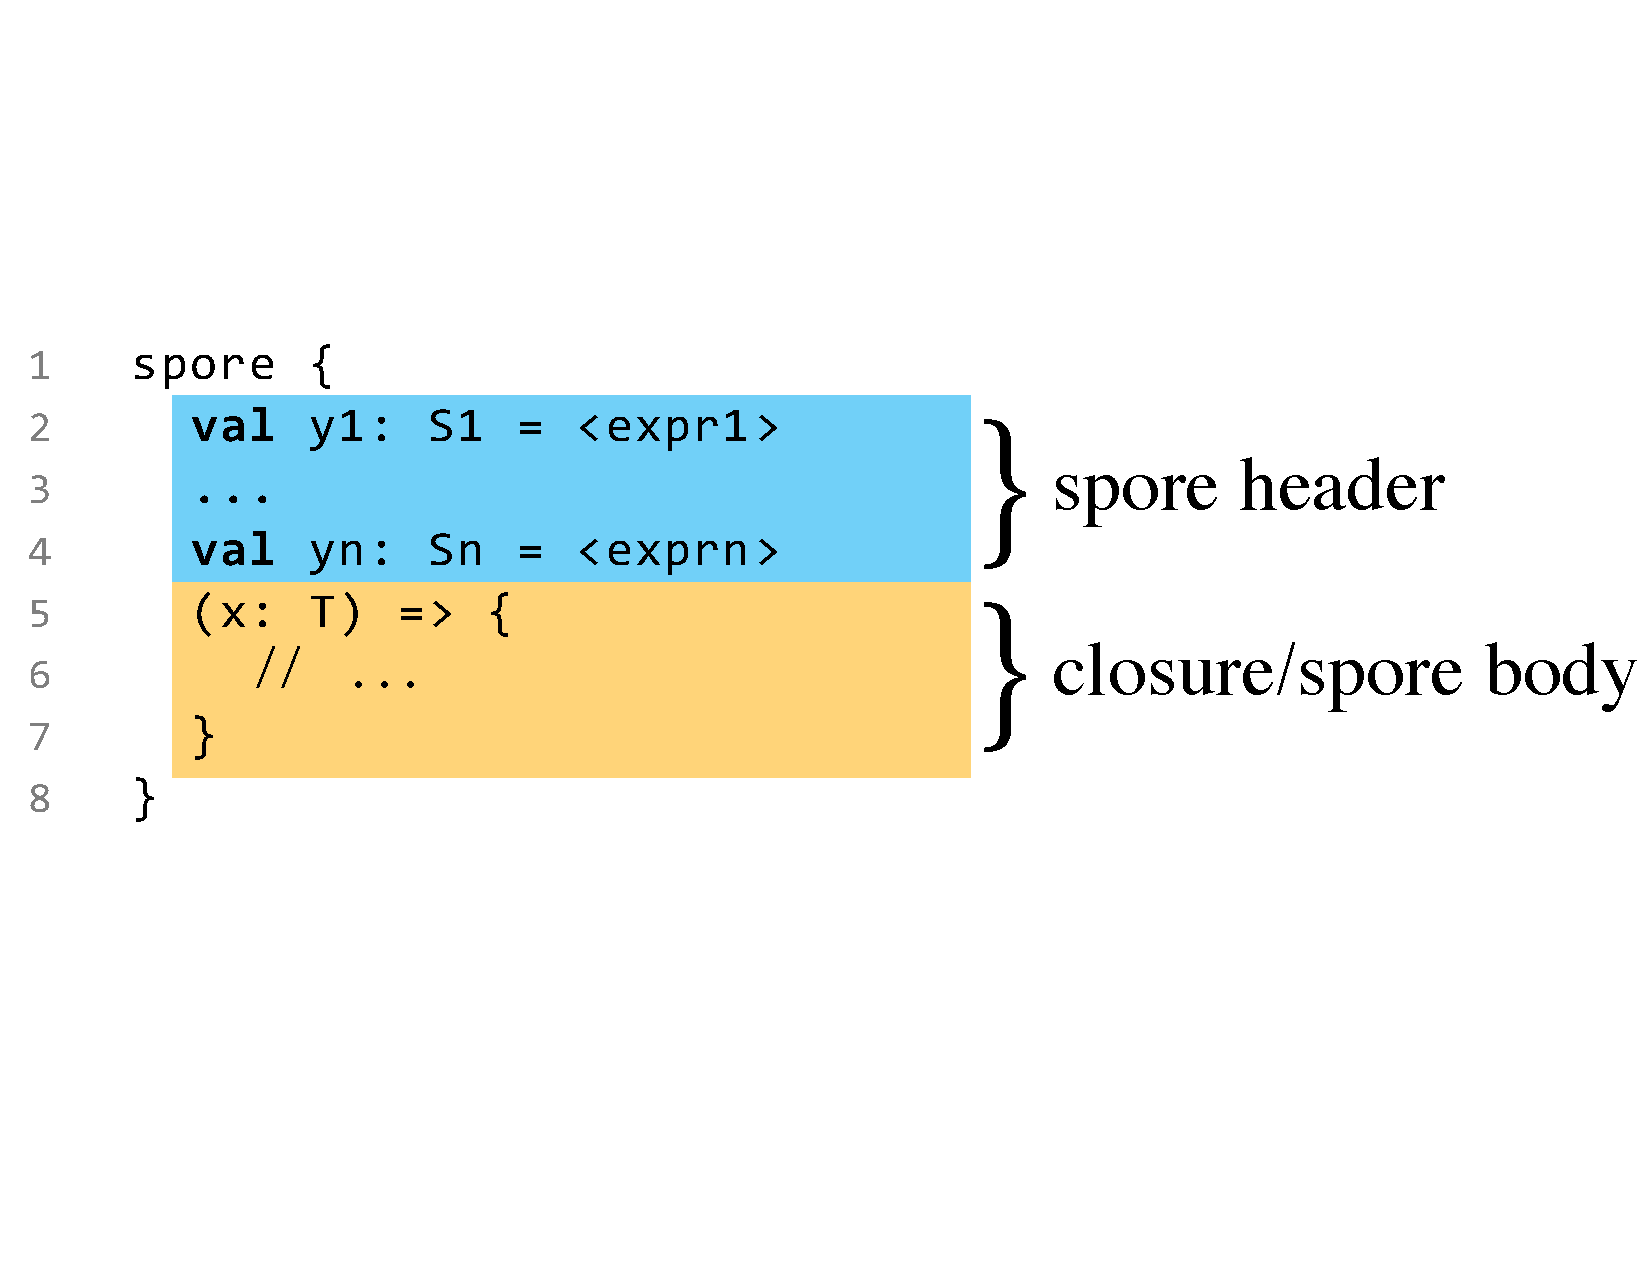
\includegraphics[width=0.75\columnwidth]{pic/spore-shape.pdf}
\end{figure}
\vspace{-1mm}

The characteristic property of a spore is that the spore body is only allowed
to access its parameter, the values in the spore header, as well as top-level
singleton objects (Scala's form of modules). The spore closure is not allowed
to capture variables other than those declared in the spore header (\ie a spore
may not capture variables in the environment). By enforcing this shape, the
environment of a spore is always declared explicitly in the spore header, which
avoids accidentally capturing problematic references. Moreover, importantly for
object-oriented languages like Scala, it's no longer possible to accidentally
capture the \verb|this| reference.

Spores also come with additional type-checking. Type information corresponding
to captured variables are included in the type of a spore. This enables authors
of distributed frameworks to customize type-checking of spores to, for example,
{\em exclude} a certain type from being captured by user-provided spores.
Authors of distributed frameworks may kick on this type-checking by simply
including information about excluded types (or other type-based properties) in
the signature of a method. A concrete example would be to ensure that the
\verb|map| method on \verb|RDD|s in Spark (a distributed collection) accepts
only spores which do not capture \verb|SparkContext| (a non-serializable
internal framework class).

For a deeper understanding of spores, see
% either Appendix~\ref{appendix:spores} which covers the semantics of spores or
the corresponding publication~\cite{Spores}.

\begin{figure}[t!]
\centering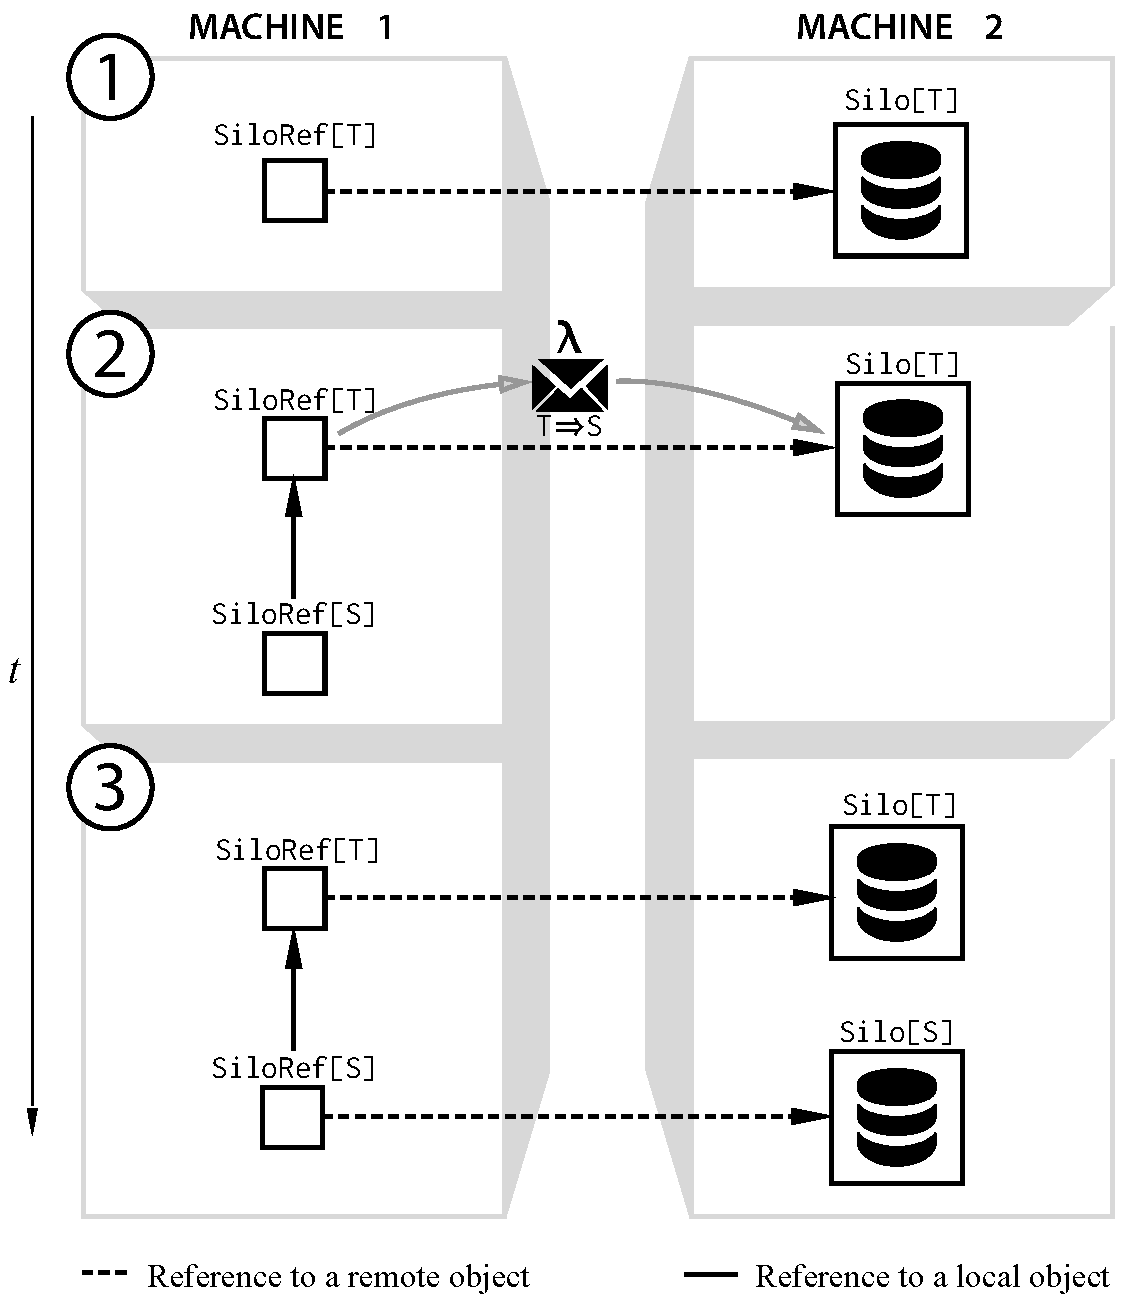
\includegraphics[width=0.8\columnwidth]{pic/basic-diagram.pdf}
\caption{Basic F-P model.}\label{fig:basic-diagram}
\end{figure}

\subsection{Basic Usage}

We begin with a simple visual example to provide a feeling for the basics of
the F-P model.\footnote{We also feel that, to visually illustrate a system
  evolving in both space and time, nothing beats a video animation. So, we've
  produced a short animation to provide visual intuition of the F-P model:
\url{https://vimeo.com/120415626}}

The only way to interact with distributed data stored in silos is through the
use of SiloRefs. A SiloRef can be thought of as an immutable handle to the
remote data contained within a corresponding silo. Users interact with this
distributed data by applying functions to SiloRefs, which are transmitted over
the wire and later applied to the data within the corresponding silo. As is the
case for persistent data structures, when a function is applied to a piece of
distributed data via a SiloRef, a SiloRef representing a new silo containing
the transformed data is returned.

The simplest illustration of the model is shown in
Figure~\ref{fig:basic-diagram} (time flows vertically from top to bottom).
Here, we start with a \verb|SiloRef[T]| which points to a piece of remote data
contained within a \verb|Silo[T]|. When the function shown as $\lambda$ of type
$T \Rightarrow S$ is applied to \verb|SiloRef[T]| and ``forced'' (sent over the
wire), a new SiloRef of type \verb|SiloRef[S]| is immediately returned. Note
that \verb|SiloRef[S]| contains a reference to its parent SiloRef,
\verb|SiloRef[T]|. (This is how {\em lineages} are constructed.) Meanwhile, the
function is asynchronously sent over the wire and is applied to \verb|Silo[T]|,
eventually producing a new \verb|Silo[S]| containing the data transformed by
function $\lambda$. This new \verb|SiloRef[S]| can be used even before its
corresponding silo is materialized (\ie before the data in \verb|Silo[S]| is
computed) – the F-P framework queues up operations applied to \verb|SiloRef[S]|
and applies them when \verb|Silo[S]| is fully materialized.

Different sorts of complex DAGs can be asynchronously built up in this way.
Though first, to see how this is possible, we need to develop a clearer idea of
the primitive operations available on SiloRefs and their semantics. We describe
these in the following section.

\begin{figure}[t!]
\centering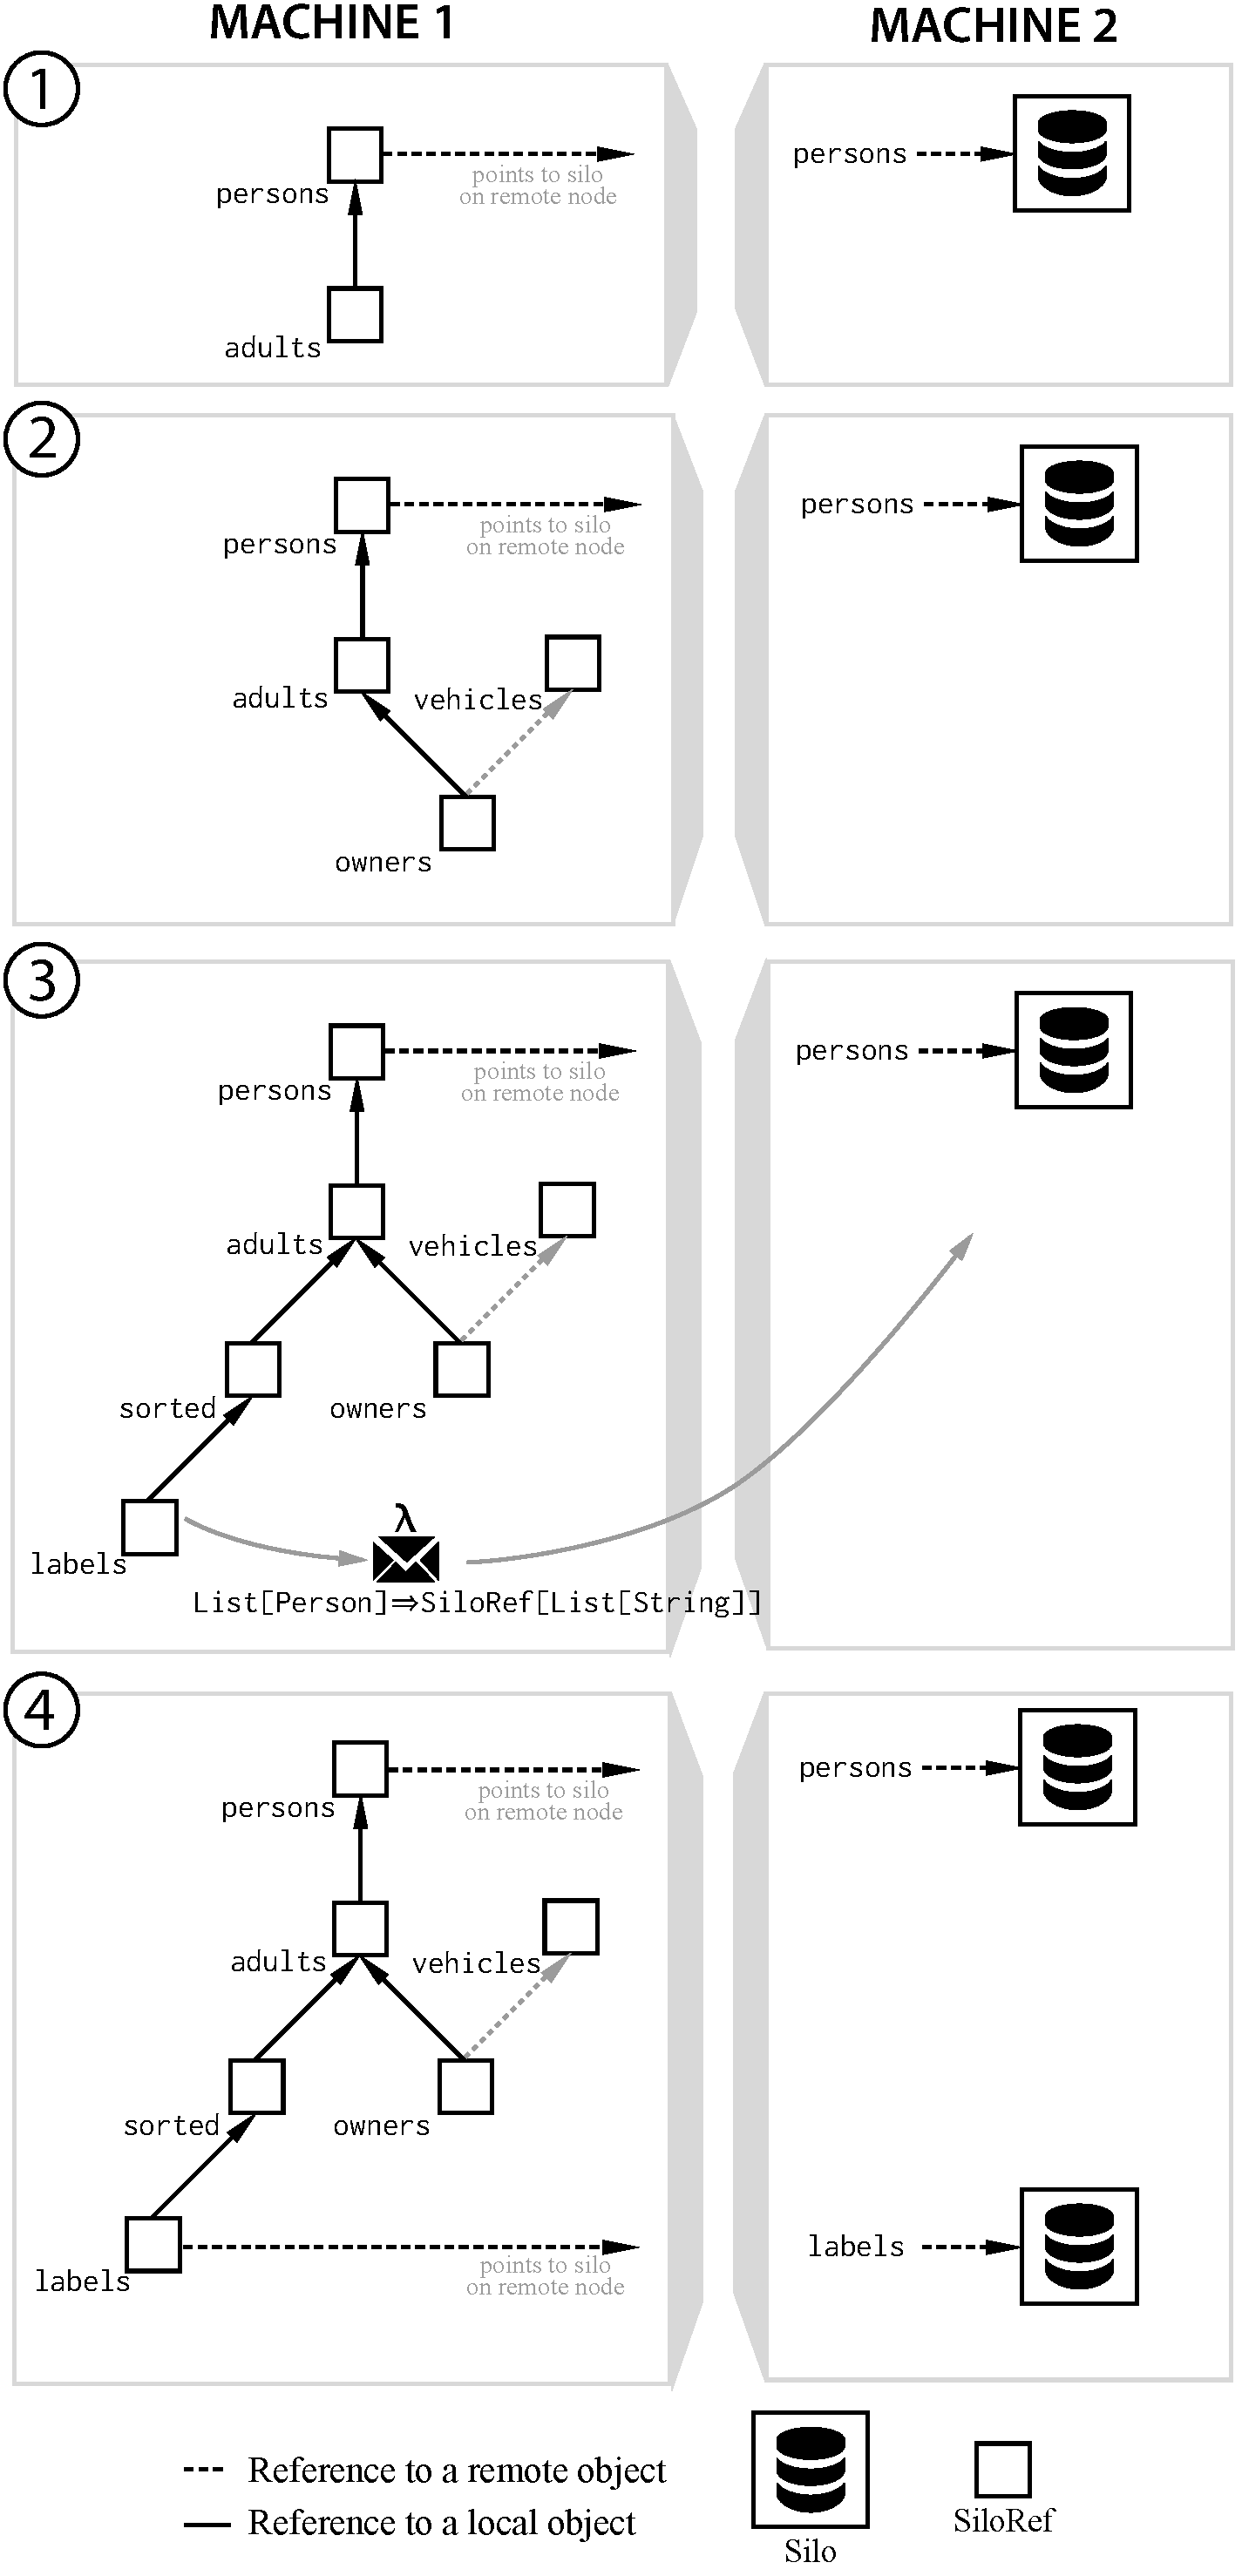
\includegraphics[width=\columnwidth]{pic/bigger-dag.pdf}
\caption{A simple DAG in the F-P model.}\label{fig:bigger-dag}
\end{figure}

\subsection{Primitives}
\label{sec:primitives}

There are four basic primitive operations on SiloRefs that together can be used
to build the higher-order operations common to popular data-centric distributed
systems (how to build some of these higher-order operations is described in
Section~\ref{sec:hoo}). In this section we'll introduce
these primitives in the context of a running example. These primitives include:

\begin{itemize}[noitemsep,nolistsep]
\item \verb|map|
\item \verb|flatMap|
\item \verb|send|
\item \verb|cache|
\end{itemize}

\paragraph{map}%
%
\texttt{def map[S](s: Spore[T, S]): SiloRef[S]} \newline 
%
The \verb|map| method takes a spore that is to be applied to the data in the
silo associated with the given SiloRef. Rather than immediately sending the
spore across the network, and waiting for the operation to finish, the
\verb|map| method is \emph{lazy}. Without involving any network communication,
it immediately returns a SiloRef referring to a new, lazily-created silo. This
new SiloRef only contains lineage information, namely, a reference to the
original SiloRef, a reference to the argument spore, and the information that
it is the result of a \verb|map| invocation. As we explain below, another
method, \verb|send| or \verb|cache|, must be called explicitly to force the
materialization of the result silo.

To better understand how DAGs are created and how remote silos are
materialized, we will develop a running example throughout this section. Given
a silo containing a list of \verb|Person| records, the following application of
\verb|map| defines a (not-yet-materialized) silo containing only the records of
adults (graphically shown in Figure~\ref{fig:bigger-dag}, part 1):

\begin{lstlisting}
val persons: SiloRef[List[Person]] = ...
val adults =
  persons.map(spore { ps => ps.filter(p => p.age >= 18) })
\end{lstlisting}

\paragraph{flatMap}%
%
\texttt{def flatMap[S](s: Spore[T, SiloRef[S]]): SiloRef[S]} \newline
%
Like \verb|map|, the \verb|flatMap| method takes a spore that is to be applied
to the data in the silo of the given SiloRef. However, the crucial difference
is in the type of the spore argument whose result type is a SiloRef in this
case. Semantically, the new silo created by \verb|flatMap| is defined to
contain the data of the silo that the user-defined spore returns.  The
\verb|flatMap| combinator adds expressiveness to our model that is essential to
express more interesting computation DAGs. For example, consider the problem of
combining the information contained in two different silos (potentially located
on different hosts). Suppose the information of a silo containing
\verb|Vehicle| records should be enriched with other details only found in the
\verb|adults| silo. In the following, \verb|flatMap| is used to create a silo
of \verb|(Person, Vehicle)| pairs where the names of person and vehicle owner
match (graphically shown in Figure~\ref{fig:bigger-dag}, part 2):

\begin{lstlisting}
val vehicles: SiloRef[List[Vehicle]] = ...
// adults that own a vehicle
val owners = adults.flatMap(spore {
  val localVehicles = vehicles // spore header
  ps =>
    localVehicles.map(spore {
      val localps = ps // spore header
      vs =>
        localps.flatMap(p =>
          // list of (p, v) for a single person p
          vs.flatMap {
            v => if (v.owner.name == p.name) List((p, v)) else Nil
          }
        )
    })
})
\end{lstlisting}
\noindent
Note that the spore passed to \verb|flatMap| declares the capturing of the
\verb|vehicles| SiloRef in its so-called ``spore header.'' The spore header
spans all variable definitions between the spore marker and the parameter list
of the spore's closure. The spore header defines the variables that the spore's
closure is allowed to access. Essentially, spores limit the free variables of
their closure's body to the closure's parameters and the variables declared in
the spore's header. Within the spore's closure, it is necessary to read the
data of the \verb|vehicles| silo in addition to the \verb|ps| list of
\verb|Person| records. This requires calling \verb|map| on
\verb|localVehicles|. However, \verb|map| returns a SiloRef; thus, invoking
\verb|map| on \verb|adults| instead of \verb|flatMap| would be impossible,
since there would be no way to get the data out of the silo returned by
\verb|localVehicles.map(..)|. With the use of \verb|flatMap|, however, the call
to \verb|localVehicles.map(..)| creates the final result silo, whose data is
then also contained in the silo returned by \verb|flatMap|.

Although the expressiveness of the \verb|flatMap| combinator subsumes that of
the \verb|map| combinator (see Section~\ref{sec:expr}), keeping \verb|map| as a
(lightweight) primitive enables more opportunities for optimizing computation
DAGs (\eg operation fusion~\cite{FlumeJava}).

\paragraph{send}%
%
\texttt{def send(): Future[T]} \newline
%
As mentioned earlier, the execution of computations built using SiloRefs is
deferred. The \verb|send| operation {\em forces} the lazy computation defined
by the given SiloRef.  Forcing is explicit in our model, because it requires
sending the lineage to the remote node on which the result silo should be
created. Given that network communication has a latency several orders of
magnitude greater than accessing a word in main memory, providing an explicit
send operation is a judicious choice~\cite{ANoteDistComp}.

To enable materialization of remote silos to proceed concurrently, the
\verb|send| operation immediately returns a future~\cite{Futures}. This future
is then asynchronously completed with the data of the given silo. Since calling
\verb|send| will materialize a silo and send its data to the current node,
\verb|send| should only be called on silos with reasonably small data (for
example, in the implementation of an aggregate operation such as \verb|reduce|
on a distributed collection).

\paragraph{cache}% 
%
\texttt{def cache(): Future[Unit]} \newline
%
The performance of typical data analytics jobs can be increased dramatically by
caching large data sets in memory~\cite{Spark}. To do this, the silo containing
the computed data set needs to be materialized. So far, the only way to
materialize a silo that we have shown is using the \verb|send| primitive.
However, \verb|send| additionally transfers the contents of a silo to the
requesting node--too much if a large remote data set should merely be cached in
memory remotely.  Therefore, an additional primitive called \verb|cache| is
provided, which forces the materialization of the given SiloRef, returning
\verb|Future[Unit]|.

Given the running example so far, we can add another subgraph branching off of
\verb|adults|, which sorts each \verb|Person| by age, produces a \verb|String|
gretting, and then ``kicks-off'' remote computation by calling \verb|cache| and
caching the result in remote memory (graphically shown in
Figure~\ref{fig:bigger-dag}, part 3 and 4):

\begin{lstlisting}
val sorted =
  adults.map(spore { ps => ps.sortWith(p => p.age) })
val labels =
  sorted.map(spore { ps => ps.map(p => "Welcome, " + p.name) })
labels.cache()
\end{lstlisting}
\noindent
Assuming we would also cache the \verb|owners| SiloRef from the previous
example, the resulting lineage graph would look as illustrated in
Figure~\ref{fig:all-silorefs}\todo{Figure missing?}. Note that \verb|vehicles|
is not a regular parent in the lineage of \verb|owners|; it is an indirect
input used to compute \verb|owners| by virtue of being {\em captured} by the
spore used to compute \verb|owners|.

% For example, Figure ?? shows the effect of invoking
% \verb|send| on the \verb|labels| SiloRef from above.

% The \verb|send| operation can also be used to simply cache a silo in main
% memory, for example, because the silo is known to be accessed subsequently:

% \paragraph{cache}
%
% The \verb|cache| method can be provided for convenience. It invokes
% \verb|send| not directly on the given SiloRef (which would transfer all data
% of the silo to the current node); instead, it first uses \verb|flatMap| to
% create a new silo that will be completed with the trivial value (e.g., a
% Boolean constant) of the \verb|DoneSiloRef| singleton object. Essentially,
% invoking \verb|send| on this trivial SiloRef causes the resulting future to
% be completed as soon as \verb|this| SiloRef has been materialized in main
% memory.

\subsubsection{Creating Silos}
\label{sec:creating-silos}

Besides a type definition for SiloRef, our framework also provides a companion
singleton object (Scala's form of modules). The singleton object provides
factory methods for obtaining SiloRefs referring to silos populated with some
initial data:\footnote{For clarity, only method signatures are shown.}

\begin{lstlisting}
object SiloRef {
  def fromTextFile(host: Host)(file: File): SiloRef[List[String]]
  def fromFun[T](host: Host)(s: Spore[Unit, T]): SiloRef[T]
  def fromLineage[T](host: Host)(s: SiloRef[T]): SiloRef[T]
}
\end{lstlisting}
\noindent
Each of the factory methods has a \verb|host| parameter that specifies the
target host (address/port) on which to create the silo. Note that the
\verb|fromFun| method takes a spore closure as an argument to make sure it can
be serialized and sent to \verb|host|. In each case, the returned SiloRef
contains its \verb|host| as well as a host-unique identifier. The
\verb|fromLineage| method is particularly interesting as it creates a copy of a
previously existing silo based on the lineage of a SiloRef \verb|s|. Note that
only the SiloRef is necessary for this operation to successfully complete; the
silo originally hosting \verb|s| might already have failed.

\subsubsection{Expressiveness}
\label{sec:expr}

\paragraph{Expressing \texttt{map}}

Leveraging the above-mentioned methods for creating silos, it is possible to
express \verb|map| in terms of \verb|flatMap|:

\begin{lstlisting}
def map[S](s: Spore[T, S]): SiloRef[S] =
  this.flatMap(spore {
    val localSpore = s
    (x: T) =>
      val res = localSpore(x)
      SiloRef.fromFun(currentHost)(spore {
        val localRes = res
        () => localRes
      })
  })
\end{lstlisting}
\noindent
This should come as no surprise, given that \verb|flatMap| is the monadic bind
operation on SiloRefs, and \verb|SiloRef.fromFun| is the monadic return
operation. The reason why \verb|map| is provided as one of the main operations
of SiloRefs is that direct uses of \verb|map| enable an important optimization
based on operation fusion.

\paragraph{Expressing \texttt{cache}}

The \verb|cache| operation can be expressed using \verb|flatMap| and
\verb|send|:

\begin{lstlisting}
def cache(): Future[Unit] = this.flatMap(spore {
 val localDoneSiloRef = DoneSiloRef
 res => localDoneSiloRef
}).send()

\end{lstlisting}
\noindent
Here, we first use \verb|flatMap| to create a new silo that will be completed
with the trivial value of the \verb|DoneSiloRef| singleton object (\eg
\verb|Unit|). Essentially, invoking \verb|send| on this trivial SiloRef causes
the resulting future to be completed as soon as \verb|this| SiloRef has been
materialized in memory.

% This optimization is explained following the
% discussion of the third main operation of SiloRefs, \verb|send|.

% The type \verb|SiloRef[T]| has the following main operations:

% \begin{lstlisting}
% trait SiloRef[T] {
%   def map[S](s: Spore[T, S]): SiloRef[S]
%   def flatMap[S](s: Spore[T, SiloRef[S]]): SiloRef[S]
%   def send(): Future[T]
% }
% \end{lstlisting}

\subsection{Fault Handling}
\label{sec:fault-handling}

F-P includes overloaded variants of the primitives discussed so far which
enable the definition of flexible fault handling semantics. The main idea is to
specify fault handlers for \emph{subgraphs of computation DAGs}. Our guiding
principle is to make the definition of the failure-free path through a
computation DAG as simple as possible, while still enabling the handling of
faults at the fine-granular level of individual SiloRefs.

\paragraph{Defining fault handlers}

Fault handlers may be specified whenever the lineage of a SiloRef is extended.
For this purpose, the introduced \verb|map| and \verb|flatMap| primitives are
overloaded. For example, consider our previous example, but extended with a
fault handler:

\begin{lstlisting}
val persons: SiloRef[List[Person]] = ...
val vehicles: SiloRef[List[Vehicle]] = ...
// copy of `vehicles` on different host `h`
val vehicles2 = SiloRef.fromFun(h)(spore {
  val localVehicles = vehicles
  () => localVehicles
})

val adults =
  persons.map(spore { ps => ps.filter(p => p.age >= 18) })

// adults that own a vehicle
def computeOwners(v: SiloRef[List[Vehicle]]) =
  spore {
    val localVehicles = v
    (ps: List[Person]) => localVehicles.map(...)
  }

val owners: SiloRef[List[(Person, Vehicle)]] =
  adults.flatMap(computeOwners(vehicles),
                 computeOwners(vehicles2))
\end{lstlisting}

Importantly, in the \verb|flatMap| call on the last line, in addition to
\verb|computeOwners(vehicles)|, the regular spore argument of \verb|flatMap|,
\verb|computeOwners(vehicles2)| is passed as an additional argument. The second
argument registers a \emph{failure handler} for the subgraph of the computation
DAG starting at \verb|adults|. This means that if during the execution of
\verb|computeOwners(vehicles)| it is detected that the \verb|vehicles| SiloRef
has failed, it is checked whether the SiloRef that the higher-order combinator
was invoked on (in this case, \verb|adults|) has a failure handler registered.
In that case, the failure handler is used as an alternative spore to compute
the result of \verb|adults.flatMap(..)|. In this example, we specified
\verb|computeOwners(vehicles2)| as the failure handler; thus, in case
\verb|vehicles| has failed, the computation is retried using \verb|vehicles2|
instead.
